\documentclass[tikz,border=8pt]{standalone}
% Estilos del modelo C4 para TikZ (colores y formas de C4). Los tres diagramas del informe los cargan con \input.
\usepackage{fontspec}
\usepackage{xcolor}
\usetikzlibrary{shapes.geometric,arrows.meta,positioning,calc,fit,backgrounds}
\renewcommand{\familydefault}{\sfdefault}
\hyphenpenalty=10000 \exhyphenpenalty=10000 % sin guiones al partir las palabras en las cajas

\definecolor{c4persona}{HTML}{08427B}   \definecolor{c4personab}{HTML}{073B6F}
\definecolor{c4sistema}{HTML}{1168BD}   \definecolor{c4sistemab}{HTML}{0B4884}
\definecolor{c4externo}{HTML}{999999}   \definecolor{c4externob}{HTML}{6B6B6B}
\definecolor{c4cont}{HTML}{438DD5}      \definecolor{c4contb}{HTML}{3C7FC0}
\definecolor{c4comp}{HTML}{85BBF0}      \definecolor{c4compb}{HTML}{78A8D8}

% \elem{Nombre}{[Tipo: tecnología]}{Descripción}: el texto de un elemento en tres líneas, como en C4.
\newcommand{\elem}[3]{\textbf{#1}\\[1pt]{\scriptsize #2}\if\relax\detokenize{#3}\relax\else\\[3pt]{\scriptsize #3}\fi}

\tikzset{
  c4box/.style={draw, rounded corners=4pt, align=center, inner sep=5pt, text=white, font=\sffamily\small,
                text width=3.1cm, minimum height=2.0cm},
  persona/.style={c4box, fill=c4persona, draw=c4personab},
  sistema/.style={c4box, fill=c4sistema, draw=c4sistemab},
  externo/.style={c4box, fill=c4externo, draw=c4externob},
  contenedor/.style={c4box, fill=c4cont, draw=c4contb},
  componente/.style={c4box, fill=c4comp, draw=c4compb, text=black},
  basedatos/.style={contenedor, shape=cylinder, shape border rotate=90, aspect=0.16, minimum height=2.4cm},
  limite/.style={draw=c4externob, dashed, rounded corners=6pt, inner sep=0.45cm},
  rel/.style={-{Stealth[length=2.4mm,width=1.9mm]}, line width=0.7pt, color=black!70},
  etq/.style={fill=white, inner sep=1.5pt, align=center, font=\sffamily\scriptsize, text=black!85},
}

% Cabeza de una persona (se dibuja detrás de su caja): \cabeza{nombre de la caja}
\newcommand{\cabeza}[1]{\begin{scope}[on background layer]\node[circle, fill=c4persona, draw=c4personab, minimum size=0.9cm] at ([yshift=0.18cm]#1.north) {};\end{scope}}

\begin{document}
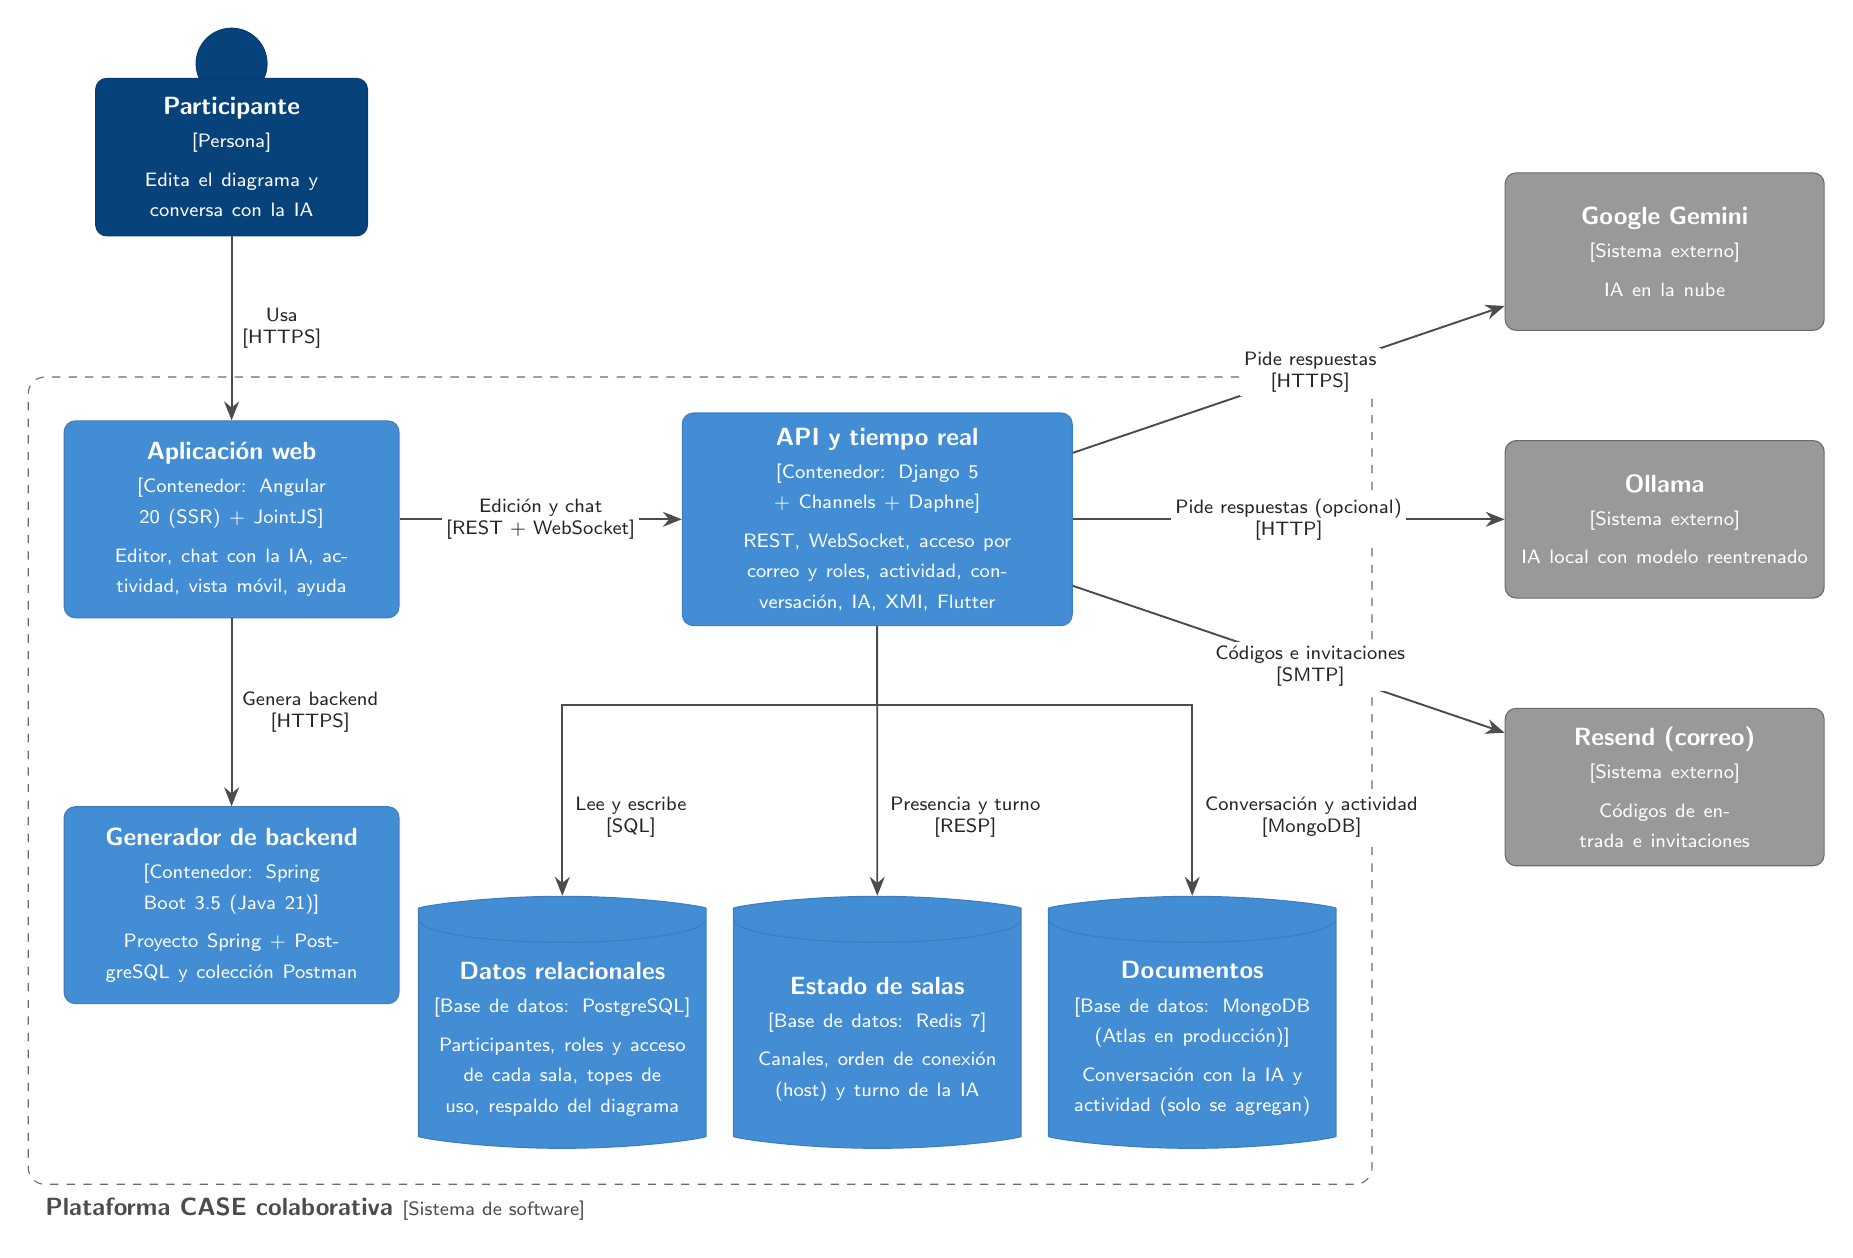
\begin{tikzpicture}
  \node[persona] (p) at (0, 4.6) {\elem{Participante}{[Persona]}{Edita el diagrama y conversa con la IA}};
  \cabeza{p}

  \node[contenedor, text width=3.9cm, minimum height=2.5cm] (web) at (0, 0) {\elem{Aplicación web}{[Contenedor: Angular 20 (SSR) + JointJS]}{Editor, chat con la IA, actividad, vista móvil, ayuda}};
  \node[contenedor, text width=4.6cm, minimum height=2.7cm] (api) at (8.2, 0) {\elem{API y tiempo real}{[Contenedor: Django 5 + Channels + Daphne]}{REST, WebSocket, acceso por correo y roles, actividad, conversación, IA, XMI, Flutter}};
  \node[contenedor, text width=3.9cm, minimum height=2.5cm] (gen) at (0,-4.9) {\elem{Generador de backend}{[Contenedor: Spring Boot 3.5 (Java 21)]}{Proyecto Spring + PostgreSQL y colección Postman}};
  \node[basedatos, text width=3.3cm, minimum height=3.2cm] (pg) at (4.2,-6.6) {\elem{Datos relacionales}{[Base de datos: PostgreSQL]}{Participantes, roles y acceso de cada sala, topes de uso, respaldo del diagrama}};
  \node[basedatos, text width=3.3cm, minimum height=3.2cm] (rd) at (8.2,-6.6) {\elem{Estado de salas}{[Base de datos: Redis 7]}{Canales, orden de conexión (host) y turno de la IA}};
  \node[basedatos, text width=3.3cm, minimum height=3.2cm] (mg) at (12.2,-6.6) {\elem{Documentos}{[Base de datos: MongoDB (Atlas en producción)]}{Conversación con la IA y actividad (solo se agregan)}};
  \node[externo, text width=3.7cm] (g) at (18.2, 3.4) {\elem{Google Gemini}{[Sistema externo]}{IA en la nube}};
  \node[externo, text width=3.7cm] (o) at (18.2, 0) {\elem{Ollama}{[Sistema externo]}{IA local con modelo reentrenado}};
  \node[externo, text width=3.7cm] (c) at (18.2,-3.4) {\elem{Resend (correo)}{[Sistema externo]}{Códigos de entrada e invitaciones}};

  % límite del sistema (rodea todo lo que está dentro de la plataforma)
  \begin{scope}[on background layer]
    \node[limite, fit=(web)(api)(gen)(pg)(rd)(mg)] (lim) {};
  \end{scope}
  \node[anchor=north west, font=\sffamily\small\bfseries, text=black!70] at ([xshift=0.1cm,yshift=-0.05cm]lim.south west) {Plataforma CASE colaborativa \normalfont\scriptsize [Sistema de software]};

  \draw[rel] (p) -- node[etq, anchor=west, pos=0.5, xshift=2pt] {Usa\\{[HTTPS]}} (web);
  \draw[rel] (web) -- node[etq, pos=0.5] {Edición y chat\\{[REST + WebSocket]}} (api);
  \draw[rel] (web) -- node[etq, anchor=west, pos=0.5, xshift=2pt] {Genera backend\\{[HTTPS]}} (gen);
  \draw[rel] (api.south) -- ++(0,-1.0) -| (pg.north);
  \draw[rel] (api) -- (rd);
  \draw[rel] (api.south) -- ++(0,-1.0) -| (mg.north);
  \node[etq, anchor=west] at ([xshift=3pt,yshift=1.0cm]pg.north) {Lee y escribe\\{[SQL]}};
  \node[etq, anchor=west] at ([xshift=3pt,yshift=1.0cm]rd.north) {Presencia y turno\\{[RESP]}};
  \node[etq, anchor=west] at ([xshift=3pt,yshift=1.0cm]mg.north) {Conversación y actividad\\{[MongoDB]}};
  \draw[rel] (api) -- node[etq, pos=0.55] {Pide respuestas\\{[HTTPS]}} (g);
  \draw[rel] (api) -- node[etq, pos=0.5] {Pide respuestas (opcional)\\{[HTTP]}} (o);
  \draw[rel] (api) -- node[etq, pos=0.55] {Códigos e invitaciones\\{[SMTP]}} (c);
\end{tikzpicture}
\end{document}
